%!TEX root = draft.tex

\section{Convergent Return-Value Consistency}
\label{sec:specifications and consistencies}

%In this section, we introduce our formation of specification. Then, we propose strong-return-value consistency, which is a sub-notion of eventual consistency of \cite{Bouajjani:2014} that strengthen the ``safety part'' specific for intuition of CRDT algorithms and ignores the ``liveness part''.




%\subsection{Specification}
%\label{subsec:specification}

%Given

%\begin{itemize}
%\setlength{\itemsep}{0.5pt}
%\item[-] $\mathbb{M}$ be a finite set of method names,

%\item[-] $\mathbb{D}$ be a possibly infinite set of data domain for argument and return values,

%\item[-] $\mathbb{R}$ be a finite set of replica identifiers, and

%\item[-] $\mathbb{O}$ be a infinite set of operation identifiers.
%\end{itemize}

%\todo{Define ``operation label'' which is $m(a,b)$ and denote operation labels by $\ell$. Operation content is not a good name.}

Let us start our formal development by introducing the definitions
required to specify CRDTs.
%
We will consider a finite set $\mathbb{M}$ of method names; and a possibly
infinite set $\mathbb{D}$ of argument and return values, the data
domain.
%
We consider replicated data types which are distributed across a set
of replicas; the set of replica identifiers is denoted by $\mathbb{R}$.
We assume that each replica contains a copy of the data type state.
Finally we have a infinite set $\mathbb{O}$ of operation identifiers,
corresponding to each individual operation performed on the CRDT
throughout an execution.
%

Operation labels \mbox{$m(a)\Rightarrow b$} with $m \in \mathbb{M}$ and $a,b \in
\mathbb{D}$, indicate that the operation is a call to method $m$
with argument $a$ and the result of the operation is the value
$b$.
When $m$ does not use the argument (resp., return value), we write
$m()\Rightarrow b$ (resp., $m(a)$) instead.
We define an operation $o$ to be a tuple $(\ell,r,i)$, where $\ell$ is
an operation label, $r \in \mathbb{R}$ is the identifier of the
replica to which the operation is submitted by the client, and $i \in \mathbb{O}$ is a
unique operation identifier.
%This definition extends naturally to the case when there are more than one arguments.
We denote by $\mathit{lab}(o)$ the label $\ell$ whenever $o = (\ell,
r, i)$.
%
Without loss of generality we will consider that the methods in
$\mathbb{M}$ can be separated in two disjoint sets of $\mathbb{Q}$
query methods, and $\mathbb{U}$ update methods.

As customary, to capture the notion of client-observable effects of an
execution over a CRDT, we will define the notion of \emph{history}.
%
A history contains a set of operations, and the order in which
they were effected in each replica.
%
Formally, a history $h$ is a tuple of the form $h = (O,\mathit{ro})$
where $O$ is a set of operations, and $\mathit{ro}$ is the replica
order.
%
For each replica $r \in \mathbb{R}$, $\mathit{ro}|_{r}$ (that is the
projection of $ro$ to operations of replica $r$) is an irreflexive
total order over all the operations with replica identifier $r$.
%
We require $\mathit{ro}$ to not relate operations with different replica identifier.
%
We also require that for each operation $o \in O$,
$\mathit{ro}^{-1}(o)$ is finite, meaning that the past of any replica
is only finite.
\fxwarning*{Check that everything is defined before}{\color {red}
An example of a history of a CRDT of list is shown in
\figurename~\ref{fig:history, annotated history and operation context} (a).
The $\mathit{add}(a,1)$ operation intends to add element $a$
on position 1 of the list of current replica, and $\mathit{read}(b\cdot a \cdot c)$ operations returns a snapshot of the list, e.g., $r\Rightarrow b\cdot a \cdot c$. These operations are submitted to two replicas.}

While histories provide the means to describe the behaviors of CRDTs,
they are insufficient to describe the effects of the delivery
policy among different replicas.
%
In other words, when does an operation become visible to another
replica, and therefore to all operations being issued at that replica?
%
This is an important notion, since specifications sometimes rely on a
certain delivery for their correctness.
%
To deal with this issue we will augment histories with additional
information, indicating when operations become visible to other
operations (i.e. the replica in which they are generated), and we
shall call them \emph{annotated histories}.
%

An annotated history $ah$ is a tuple $ah = (O,\mathit{vis},\mathit{arb})$, where
$O$ is a set of operations; $\mathit{vis}$, the visibility relation, is
an irreflexive and acyclic relation over $O$ representing for each
operation the set of operations which can affect its result
(essentially for $o$, these are the operations that are in
$\mathit{vis}^{-1}(o)$); and $\mathit{arb}$, the arbitration order, is
an irreflexive total order over a subset of the update operations of
$O$.
An important aspect of CRDTs is that in the presence of conflicting
operations (that is operations which if executed in different order
change the resulting behavior), the convergence mechanism of the CRDT
will determine the order in which the operations should be applied by
all replicas, hence guaranteeing convergence.
The order $\mathit{arb}$ plays this role in the definition of
annotated histories.
\fxnote{GP: Why only update at this point?. Add the cite to Burckhardt.} \fxwarning{GP: \c@Chao explain or remove}
{\color {red}The annotated history for history of \figurename~\ref{fig:history, annotated history and operation context} (a) is given in \figurename~\ref{fig:history, annotated
history and operation context} (b). Here we use arbitration order $\mathit{add}(b,1) < \mathit{add}(a,1) < \mathit{add}(c,1) < \mathit{add}(d,4))$.} 
%

% {\color {red} Visibility relation tells how update operations are
%   delivered, and arbitration order represents some global orders that
%   are used to determine return values on each replica, such as list
%   order in \cite{Attiya:2016} or time stamp order.}
% We further require that for each operation $o \in O$, $\mathit{vis}^{-1}(o)$ is finite.

%\fxwarning{GP: \c@Chao explain or remove}
%{\color {red}The annotated history for history of \figurename~\ref{fig:history, annotated history and operation context} (a) is given in \figurename~\ref{fig:history, annotated
%history and operation context} (b). $(\mathit{add}(a,1),\mathit{add}(d,4))$ in visibility represents that $\mathit{add}(a,1)$ is visible when submitting $\mathit{add}(d,4))$.} % with arbitration order $\mathit{add}(b,1) \cdot \mathit{add}(c,2) \cdot \mathit{add}(a,1)$.}

%\begin{itemize}
%\setlength{\itemsep}{0.5pt}
%\item[-] $O$ is a set of operations.

%\item[-] $\mathit{vis}$ is a irreflexive and acyclic relation over $O$, and is called the visibility relation. We require that for each operation $o \in O$, $\mathit{vis}^{-1}(o)$ is finite.

%\item[-] $\mathit{arb}$ is a partial order over update operations of $O$ and is called the arbitration order.
%\item[-] $\mathit{arb}$ is a irreflexive total order over a subset of update operations of $O$ and is called the arbitration order.
%\end{itemize}


\begin{figure}[t]
  \centering
  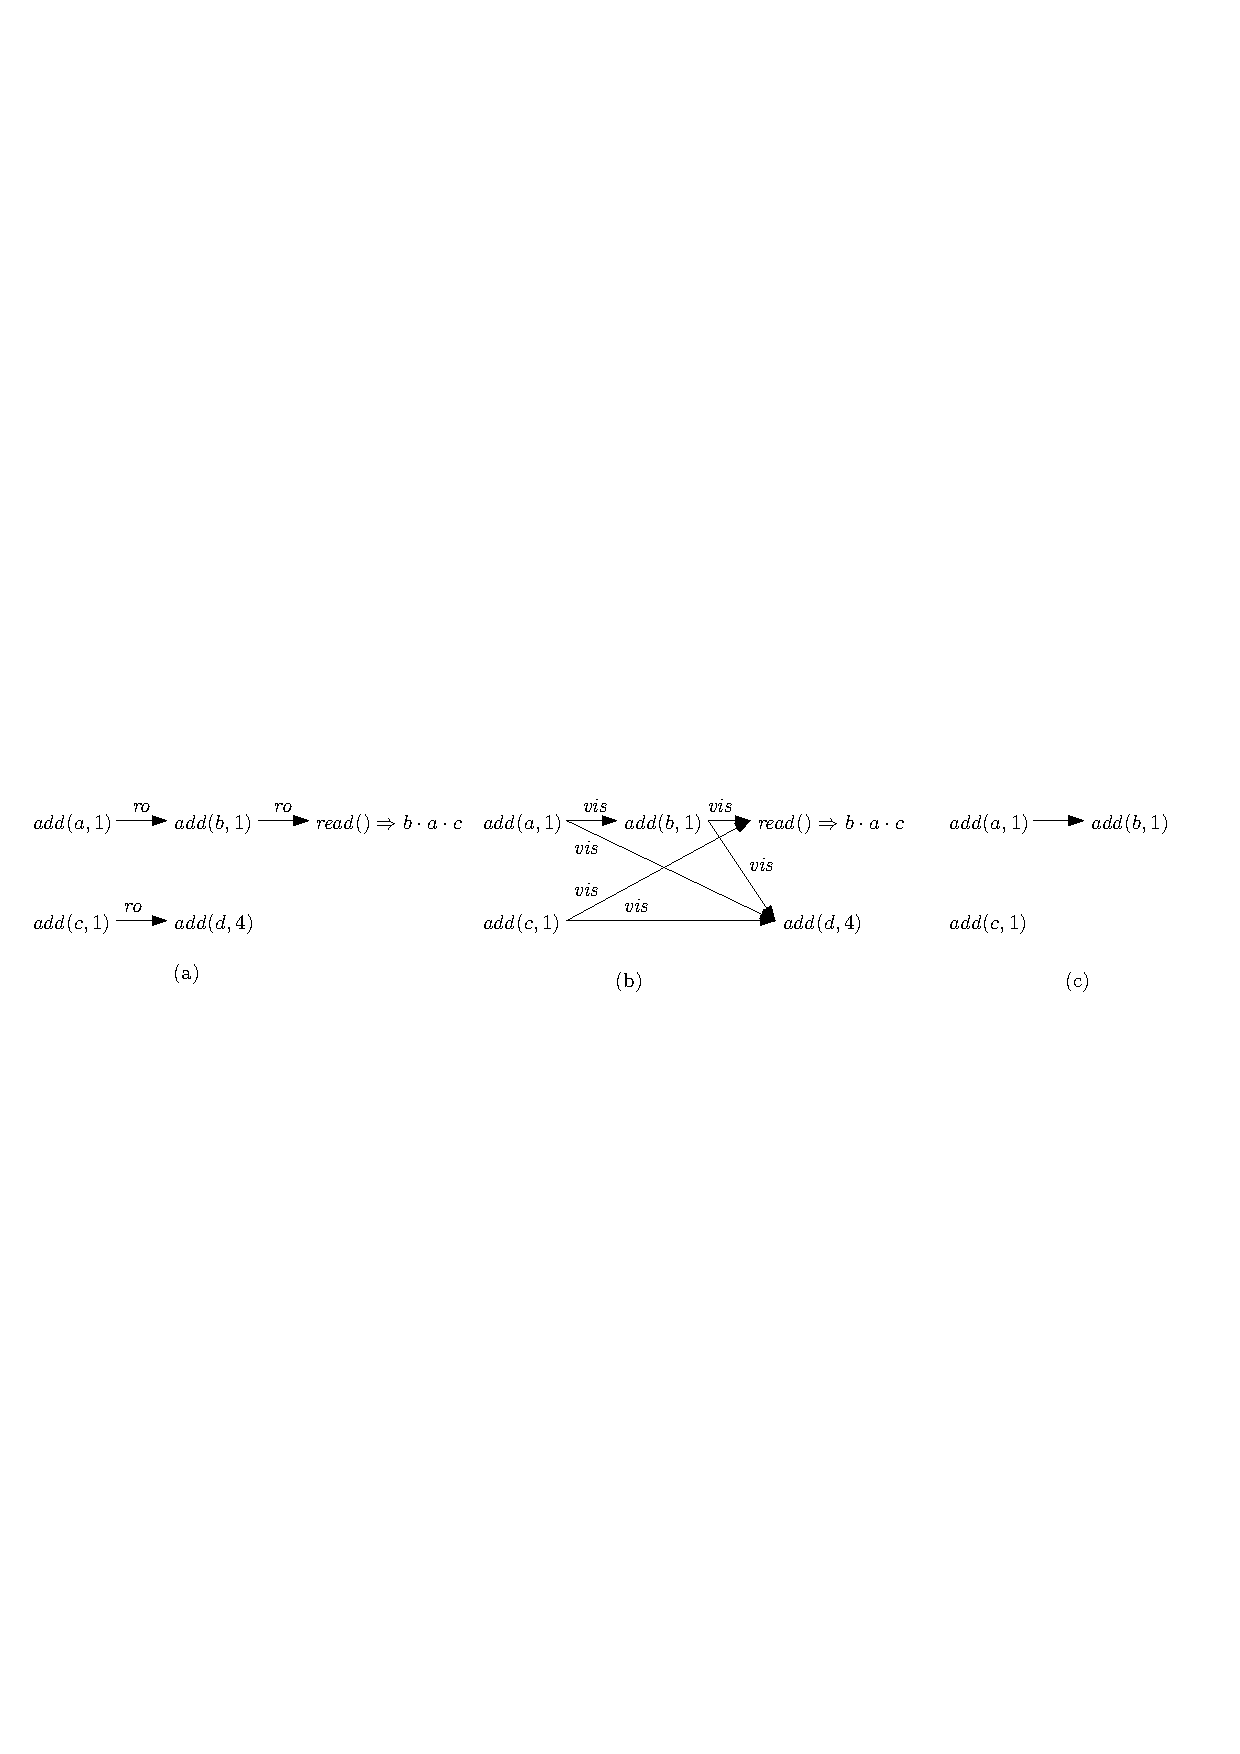
\includegraphics[width=0.9 \textwidth]{figures/PIC-his-anhis-context-1.pdf}
%\vspace{-10pt}
  \caption{{\color {red}A history of list, its annotated history, and an operation context of $\mathit{add}(d,4)$.}}

  %Here $+(a,1)$ represents $\mathit{add}(a,1)$, $r(b \cdot a \cdot c)$ represents $\mathit{read}(b \cdot a \cdot c)$; $+a_1$ and $-a_1$ represents $\mathit{add}(a)$ and $\mathit{rem}(a)$, respectively, while the subscript number is used to distinguish different $\mathit{add(a)}$; $(a,\surd)$ represents $\mathit{contains}(a,\mathit{true})$. In annotated history (b), we use arbitration order $\mathit{add}(b,1) \cdot \mathit{add}(a,1) \cdot \mathit{add}(c,1) \cdot \mathit{add}(d,4)$. Assume that the visibility relation contains the replica order.}
  \label{fig:history, annotated history and operation context}
\end{figure}


Following~\cite{Burckhardt:2014} we provide the formal specification of
CRDT by means of a specification function $\mathit{Spec}$ which takes
an operation name, a set of arguments corresponding to the arity and
the types of the operation, and a \emph{context} representing the
information available to the replica executing the operation.
Provided with these parameters, $\mathit{Spec}$ returns a single value
that results from executing the operation.
%
The context of an operation $o$ here is a triple of the form
$(O,<,\mathit{arb})$, where $O$ is a set of update operations, $<$ is
a pre-order a subset of $O$ such that $o \notin O$ and $\mathit{arb}$
is an irreflexive total order over a subset of the update
operations\footnote{Notice that unlike~\cite{Burckhardt:2014}, we
  consider that $o \notin O$. } of $O \cup \{o\}$.
%
\fxnote{GP: Have no idea why!}
%
The intuitive meaning of the relation $<$ is that encodes the
happens-before relation~\cite{Lamport:1978} over the updates that are
visible to the operating through $\mathit{vis}$.

We can now formally define the specification function $\mathit{Spec}$
as in~\cite{Burckhardt:2014}.
$\mathit{Spec}$ takes an operation name $m \in \mathbb{B}$, arguments
$a$, and a context $(O, <, \mathit{arb})$, and it returns a value $b$
(written $\mathit{Spec}(m, a, (O, <, \mathit{arb})) = b$).
%
Moreover, assuming that the resulting operation from the call to
$m(a)$ will be given the operation identifier $o \in \mathbb{O}$, we
assume that $o\notin O$ (hence $lab(o) = m(a) \Rightarrow b$), and
that $o$ can occur in $\mathit{arb}$.
%
We shall in the rest of the paper overload the function name
$\mathit{Spec}$ parameterized by labels, and adopt the notation
\mbox{$Spec(m(a) \Rightarrow b)$} to denote the set of contexts that
generate that label, that is:
\[Spec(m(a) \Rightarrow b) \triangleq \{\ (O, <, \mathit{arb})\ |\
  Spec(m, a, (O, <, \mathit{arb})) = b\ \}\]
%
%We recall at this point that since specifications are deterministic,
%$\mathit{Spec}$ is a %%functi.

% As in~Burkhardt:2014} we require specifications to be deterministic.
% {\color {red}Similarly as in \cite{Burckhardt:2014}, in defining specification, we use the notion of operation context, which contains all information necessary to ensure the correctness of an operation.} A operation context of a operation $o$ is a tuple $(O,<,\mathit{arb})$, where $O$ is a set of update operations, $<$ is a relation over $O$, $o \notin O$, and $\mathit{arb}$ is a irreflexive total order over a subset of update operations of $O \cup \{ o \}$. {\color {red}Here we modified that of \cite{Burckhardt:2014} by making $o \notin O$ itself also contained in the arbitration order. This feature is used to deal with list specification.} A specification $\mathit{Spec}$ is a function that maps each operation label $\ell$ into a set of elements, while each of them is a operation context $(O,<,\mathit{arb})$ for some operation $o$ with $\mathit{lab}(o) = \ell$. {\color {red}


% A specification is deterministic, if there does not exists query
% method $m$ and tuple $(O,<,\mathit{arb})$, such that
% $(O,<,\mathit{arb})$ is in both $\mathit{Spec}(m(a) \Rightarrow b)$
% and $\mathit{Spec}(m(a') \Rightarrow b')$, and $a \neq a' \vee b \neq
% b'$.
% From now on, we consider only deterministic specifications.

Given an annotated history $ah = (O,\mathit{vis},\mathit{arb})$ and an
operation $o \in O$, we define the context extracting function $ctxt(ah, o)$
which returns a context $(O', <, \mathit{arb'})$ such that:
\begin{inparaenum}[(i)]
\item $O'$ is the set \emph{update} operations in $\mathit{vis}^{-1}(o)$,
\item $<$ is the projection of $\mathit{vis}$ over $O'$, and
\item $\mathit{arb'}$ is the projection of $\mathit{arb}$ over $O' \cup \{o\}$.
\end{inparaenum} Therefore, given an annotated history $ab =
(O,\mathit{vis},\mathit{arb})$ and $o_1,o_2 \in O$, if $o_1$ and $o_2$
see the same set of operations, i.e. $O_1 = O_2$, then $ctxt(o_1) = ctxt(o_2)$.
%
This is consistent with the commutativity requirement of CRDTs.
\fxwarning*{GP: @Chao explain better the examples}{For example,
  \figurename~\ref{fig:history, annotated history and operation context}
  (c) is the operation context of $o = \mathit{add}(d,4)$ in
  \figurename~\ref{fig:history, annotated history and operation context}
  (b).{\color {red} Here the operations visible to $o$ are $\{ \mathit{add}(a,a), \mathit{add}(b,1), \mathit{add}(c,1)\}$, and the arbitration order is same as that of \figurename~\ref{fig:history, annotated history and operation context}
  (b).} 
  Similarly, this definition modifies that of \cite{Burckhardt:2014}
  to deal with list.}
%
\fxfatal*{GP: No idea what this means.}{\color {red}The process of obtaining operation context from annotated history for OR-set is a little different and we discuss it in Remark \ref{remark: operation context of OR-set}.}

%Note that the uniformly
%  method of obtaining operation context from annotated history is
%  suitable for most specifications.
%  For one special case, the OR-set, we shows how to deal with it in
%  Remark \ref{remark: operation context of OR-set}.}
  % To comply with the commutativity intuition of CRDT algorithm, we further require that, given an annotated history $(O,\mathit{vis},\mathit{arb})$ and $o_1,o_2 \in O$, if $\mathit{vis}^{-1}(o_1) = \mathit{vis}^{-1}(o_2)$, then $<_1 = <_2$, where $ctxt(o_1)=(O_1,<_1,\mathit{arb}_1)$ and $ctxt(o_2)=(O_2,<_2,\mathit{arb}_2)$.

\fxfatal{GP: How is this different from RVal Consistency from~\cite{Burckhardt:2014}?}
The notion of Convergent Return-Value Consistency (CRVC, for short)
requires the return value of each operation to correspond to its
specification, and it is defined as follows:

\begin{definition}[Convergent Return-Value Consistency]
\label{definition:strong return value consistency}
An annotated history $ah = (O,\mathit{vis},\mathit{arb})$ is CRVC w.r.t specification $\mathit{Spec}$, if:
\begin{enumerate}[(i)]
\item $\mathit{vis}$ is acyclic, and
\item $\forall o \in O$, $\mathit{ctxt}(o) \in Spec(\mathit{lab}(o))$.
\end{enumerate}

Moreover, a history $h = (O,\mathit{ro})$ is CRVC w.r.t $\mathit{Spec}$, if
there exist $\mathit{vis}$ and $\mathit{arb}$, such that $\mathit{ro}
\subseteq \mathit{vis}$, and $(O,\mathit{vis},\mathit{arb})$ is CRVC
consistent w.r.t $\mathit{Spec}$.
\end{definition} 


\begin{figure}[t]
  \centering
  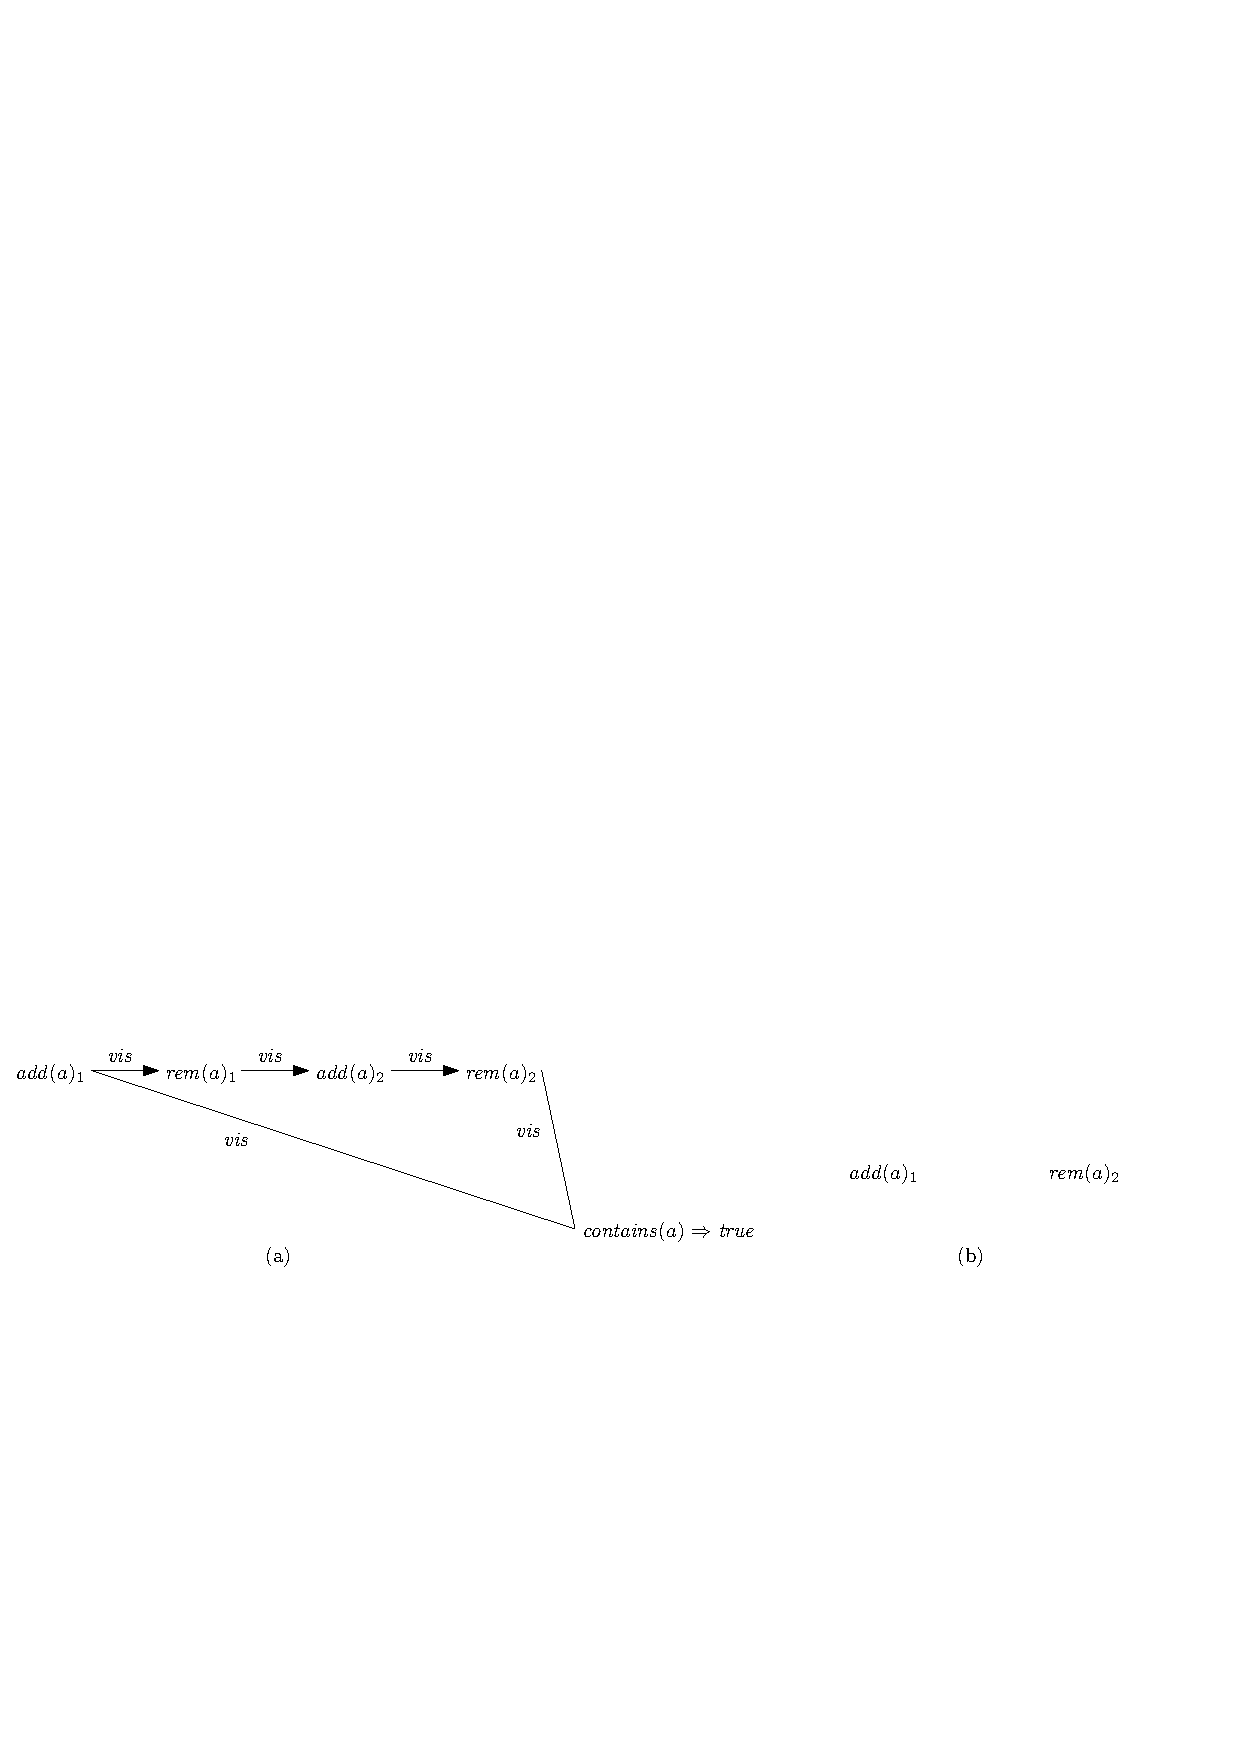
\includegraphics[width=1 \textwidth]{figures/PIC-his-anhis-context-2.pdf}
%\vspace{-10pt}
  \caption{{\color {red} Generating operation context from annotated history for OR-set.}}

  %Here $+(a,1)$ represents $\mathit{add}(a,1)$, $r(b \cdot a \cdot c)$ represents $\mathit{read}(b \cdot a \cdot c)$; $+a_1$ and $-a_1$ represents $\mathit{add}(a)$ and $\mathit{rem}(a)$, respectively, while the subscript number is used to distinguish different $\mathit{add(a)}$; $(a,\surd)$ represents $\mathit{contains}(a,\mathit{true})$. In annotated history (b), we use arbitration order $\mathit{add}(b,1) \cdot \mathit{add}(a,1) \cdot \mathit{add}(c,1) \cdot \mathit{add}(d,4)$. Assume that the visibility relation contains the replica order.}
  \label{fig:generating operation context from annotated history for OR-set}
\end{figure}




\noindent {\bf Example 1. OR-set}:
%
{\color {red} Observed-Remove Set (OR-set for short) \cite{Shapiro:2011,Bieniusa:2012} maintains the view of a set in each replica. Each $\mathit{rem}(a)$ can only cancel the $\mathit{add}(a)$ that are visible to it. Therefore, given two current (not visible to each other) operations $\mathit{add}(a)$ and $\mathit{rem}(a)$, the $\mathit{add}(a)$ take precedence.} OR-set contains four methods: (1)
$\mathit{add}(a)$ inserts $a$ into the set, (2) $\mathit{rem}(a)$
removes $a$ from set, (3) \mbox{$\mathit{lookup}(a)\Rightarrow
  \mathit{true}$} (resp., \mbox{$\mathit{lookup}(a)\Rightarrow
  \mathit{false}$}) represents the inclusion of the element $a$ in the
set (resp. its exclusion), and $\mathit{elements}() \Rightarrow S$
indicates that the contents of the set are $S$.

% \todo{Why do you need $\top$ as argument ??
%   If it's because you want to use operation labels for messages as
%   well, I don't like it.
%   Each part of the formalism should be as clear as possible, without
%   unnecessary junk.}
% Let $\Sigma_{\mathit{ORS}} = \{ add(a,\top),rem(\top,a) \vert a \in
% \mathbb{D} \}$ be the set of contents of update operations.
Given an annotated history $ah = (O, \textit{vis}, \emph{arb})$, the
specification of OR-set, $S_{\mathit{ORS}}$, is as follows:
\begin{inparaenum}[(1)]
\item $S_{\mathit{ORS}}(\mathit{add}(a))$ is the set of all tuples
  $(O,<,\emptyset)$,
\item $S_{\mathit{ORS}}(\mathit{lookup}(a) \Rightarrow \mathit{true})$
  is the set of all tuples $(O,<,\emptyset)$, such that the projection
  of $<$ over $\mathit{add}(a)$ and $\mathit{rem}(a)$ in $O$ contains a
  maximal element with operation label $\mathit{add}(a)$.
  A similar definition can be given for $\mathit{lookup}(a)
  \Rightarrow \mathit{false}$, where $O$, contains no maximal element
  with operation label $\mathit{add}(a)$,
\item $S_{\mathit{ORS}}(\mathit{rem}(a))$ is similar to
  $\mathit{lookup}(a) \Rightarrow \mathit{true}$, and
\item $S_{\mathit{ORS}}(\mathit{elements}() \Rightarrow S)$ are all
  the tuples $(O,<,\emptyset)$ that are in
  $S_{\mathit{ORS}}(\mathit{lookup}(a) \Rightarrow \mathit{true})$ for
  each $a \in S$, and are in $S_{\mathit{ORS}}(\mathit{lookup}(a)
  \Rightarrow \mathit{false})$ for each $a \notin S$.
 \end{inparaenum}
 Thus, we can observe that the specification $S_{\mathit{ORS}}$ makes
 $\mathit{rem}$ cancel only $\mathit{add}$ operations ``visible'' to
 them.
 \fxwarning*{GP: @Chao clarify}{\color {red}
 For example, \figurename~\ref{fig:generating operation context from annotated history for OR-set} (b) is in $S_{\mathit{ORS}}(\mathit{lookup}(a)
 \Rightarrow \mathit{true})$, since there is a $\mathit{add}(a)$ that is maximal w.r.t $<$. Here the subscript $1$ of $\mathit{add}(a)_1$ is used to distinguish several $\mathit{add}(a)_1$.} 

\bigskip
\noindent {\bf Example 2. Distributed list}: {\color {red} The Distributed List CRDT~\cite{Attiya:2016} mains the view of a list in each replica.} It contains three methods: (1)
$\mathit{add}(a,\mathit{pos})$ inserts value $a$ into position
$\mathit{pos} \in \mathbb{N}$ of the list, (2) $\mathit{rem}(a)$ removes the
value $a$ from the list, and (3) $\mathit{read}() \Rightarrow l$
returns the list contents.
%
We assume that each value appears at most once, and therefore we shall
call them identifiers.

%Let $\Sigma_{\mathit{list}} = \{ add(a,pos,\top),rem(\top,a) \vert a \in \mathbb{D},pos \in \mathbb{N} \}$ be the set of contents of update operations.
The specification $S_{\mathit{List}}$ of the distributed list is
defined as follows.
Given an annotated history $ah = (O,<,\mathit{arb})$, we say that $ ah
\in S_{\mathit{list}}(\ell)$, if
\begin{inparaenum}[(1)]
% \setlength{\itemsep}{0.5pt}
\item $arb$ is a total order over all of the $add$ operations in $O \cup \{ o \}$, where $o \notin O$, and
\item letting \mbox{$R = \{\ i\ |\ \exists b,
    (add(b),\_,i),(rem(b),\_,\_) \in O \}$} be the set of identifiers already removed identifiers and $\mathit{seq} =
  \mathit{arb}\!\!\!\uparrow_{( O \cup \{ o \} \setminus R)}$\footnote{We denote by $R \uparrow_{S}$ the projection $R$ on $S \times S$.} be the ``active'' list content 
  then, either
    \begin{inparaenum}[(i)]
    \item $\ell = add(a,pos) \wedge \mathit{seq}[pos] = o$,
    \item $\ell = rem(a) \wedge (add(a),\_,\_) \in O$, or
    \item $\ell = read() \Rightarrow l$, and $l$ is obtained by using $\mathit{lab}$ on $\mathit{seq}$.
    \end{inparaenum}
  \end{inparaenum}
\fxwarning{GP: Using lab on seq??}
  % \todo{Give a declarative specification of the list, like for OR-set. Descriptions which look like ``imperative programs'', e.g., "We can go through operations", "During this process".}
In a nutshell, this specification indicates that we use the list order
of strong list specification in \cite{Attiya:2016} as the arbitration
order. \fxwarning*{GP: @Chao explain?}{\color {red}
For example, \figurename~\ref{fig:history, annotated history and
  operation context} (c) is in specification of $o =
\mathit{add}(d,4)$, where no identifiers are removed, and the active list content is $\mathit{seq} = \mathit{add}(b,1) \cdot \mathit{add}(a,1) \cdot \mathit{add}(c,1) \mathit{add}(d,4)$, and $\mathit{seq}[4]$ is $o$.}  



\fxnote{Contains or lookup: gotta make up our mind.}
\fxfatal{GP: I have no idea of what this means. Has to be rewritten.}
\begin{remark}
  \label{remark: operation context of OR-set} {\color {red} The process of generating operation context of an annotated history for OR-set is more complicated, since some orders of  visibility relation need to be ignored. For instance, given the annotated history \figurename~\ref{fig:generating operation context from annotated history for OR-set} (a). Here note that visibility relation on same replica (replica order) is transitive. Then what should be the operation context $(O,<,\emptyset)$ of operation $\mathit{lookup}(a) \Rightarrow \mathit{true}$? Obviously $O = \{ \mathit{add}(a)_1, \mathit{rem}(a)_2 \}$. If we choose $<$ to be the visibility relation, then we have $(\mathit{add}(a)_1, \mathit{rem}(a)_2) \in <$. However, this is wrong, since $\mathit{rem}(a)_2$ does not cancel $\mathit{add}(a)_1$, but cancels $\mathit{add}(a)_2$ instead. To deal with this, we let $< = \emptyset$ and ignores the visibility relation between $\mathit{add}(a)_1$ and $\mathit{rem}(a)_2$. Formally, given $o_1$ with $\mathit{lab}(o_1) = \mathit{add}(a)$, let $\mathit{FstRem}(o_1)$ be the set of $\mathit{rem}(a)$ operations $o_2$, such that $o_1$ is visible to $o_2$ and their is no $\mathit{rem}(a)$ operations $o_3$ that satisfies ($(o_1,o_3),(o_3,o_2) \in \mathit{vis}$). When we generating $<$ from $\mathit{vis}$, such pairs $(o_1,o_2)$ will be ignored: $o_2 \notin \mathit{FstRem}(o_1)$, and there exists operation $o_3$, such that $(o_1,o_3),(o_3,o_2) \in \mathit{vis}$, while $o_3 \notin O$. In  \figurename~\ref{fig:generating operation context from annotated history for OR-set} (a), such ignored pair is $(\mathit{add}(a)_1,\mathit{rem}(a)_2)$, since $\mathit{rem}(a)_2 \notin \mathit{FstRem}(\mathit{add}(a)_1)$, $(\mathit{add}(a)_1,\mathit{rem}(a)_1), (\mathit{rem}(a)_1,\mathit{rem}(a)_2) \in \mathit{vis}$ while $\mathit{rem}(a_1)$ is not visible to $\mathit{lookup}(a) \Rightarrow \mathit{true}$.}
\end{remark}

\forget{


is in $S_{\mathit{ORS}}(\mathit{lookup}(a)
 \Rightarrow \mathit{true})$


 For the OR-set CRDT, the
  operation context of an annotated history is more complicated.
  For instance, given the annotated history
  \figurename~\ref{fig:history, annotated history and operation context}
  (d), the operation context of $\mathit{lookup}(a,\textit{true})$
  should be the one depicted in \figurename~\ref{fig:history, annotated
    history and operation context} (e), since $-a_2$ does not cancel
  $+a_1$, and they should not be related.
  Formally, given an annotated history $ah =
  (O,\mathit{vis},\mathit{arb})$ and an operation $o$,
  $ctxt(o)=(O',<,\mathit{arb}')$, where $O'$ and $\mathit{vis}'$ is as
  before, and $<$ is defined as $\mathit{vis} \uparrow_{O'} - \{
  (o_1,o_2) \vert o_2 \notin \mathit{FstRem}(O,\mathit{vis},o_1),$
  $\exists o_3 \in O, (o_1,o_3), (o_3,o_2),(o_1,o_2) \in \mathit{vis},
  o_1,o_2 \in O', o_3 \notin O' \}$.
  {\color {red}Here $\mathit{FstRem}$ records matched $\mathit{add}$
    and $\mathit{rem}$ pairs like $(+a_1,-a_1)$,} and is defined as
  $\mathit{FstRem}(O,\mathit{vis},o) = \{o' \vert
  \mathit{lab}(o')=\mathit{rem}(a), (o,o') \in \mathit{vis}, \neg
  \exists o'', lab(o'') = \mathit{rem}(a) \wedge (o,o''),(o'',o') \in
  \mathit{vis} \}$ for $lab(o) = \mathit{add}(a)$.
}
%{\color {red}Remark: For OR-set, the operation context of annotated history is more complicated: Given an annotated history $(O,\mathit{vis},\mathit{arb})$ and an operation $o$, $ctxt(o)=(O',<,\mathit{arb}')$, where $O'$ and $\mathit{vis}'$ is as before, and $< = \mathit{vis} \uparrow_{(O' \times O')} - \{ (o_1,o_2) \vert o_2 \notin FstRem(O,\mathit{vis},o_1), \exists o_3 \in O, (o_1,o_3), (o_3,o_2),(o_1,o_2) \in \mathit{vis}, o_1,o_2 \in O', o_3 \notin O' \}$. Here $FstRem(O,\mathit{vis},o)$ is the set of first visible matching remove of $o$ w.r.t $\mathit{vis}$, and is defined as $FstRem(O,\mathit{vis},o) = \{o' \vert lab(o')=rem(a), (o,o') \in \mathit{vis}, \neg \exists o'',  lab(o'') = rem(a)  \wedge (o,o''),(o'',o') \in \mathit{vis} \}$ for $lab(o) = add(a)$.}


%Given an annotated history $(O,\mathit{vis},\mathit{arb})$ and an operation $o$, $ctxt(o)=(O',<,\mathit{arb}')$ of OR-set is defined as follows: $\mathit{arb}' = \emptyset$, and $< = \mathit{vis} \uparrow_{(O' \times O')} - \{ (o_1,o_2) \vert o_2 \notin Minus(O,\mathit{vis},o_1), \exists o_3 \in O, (o_1,o_3), (o_3,o_2),(o_1,o_2) \in \mathit{vis}, o_1,o_2 \in O', o_3 \notin O' \}$. Here $Minus(O,\mathit{vis},o)$ is the set of first visible matching remove of $o$ w.r.t $\mathit{vis}$, and is defined as $Minus(O,\mathit{vis},o) = \{o' \vert lab(o')=rem(a), (o,o') \in \mathit{vis}, \neg \exists o'',  lab(o'') = rem(a)  \wedge (o,o''),(o'',o') \in \mathit{vis} \}$ for $lab(o) = add(a)$.




%The specification $S_{\mathit{list}}$ is defined as follows: $(O,<,arb) \in S_{\mathit{list}}(\ell)$, if

%\begin{itemize}
%\setlength{\itemsep}{0.5pt}
%\item[-] $<^{-1}$ contains finite elements, $<$ is acyclic and $arb$ is a total order of $add$ operations in $O \cup \{ o \}$, where $o \notin O$ and is in domain of $arb$.

%\item[-] {\color {red}Function $f: O \cup \{ o \} \rightarrow P(O \cup \{ o \})$. For the case of $o' \in O$, let $S(o') = f(o_1) \cup \ldots \cup f(o_k)$, where $o_1,\ldots,o_k$ is the immediate predecessor of $o'$ w.r.t $<$. Then, $f(o')$ is recursively defined as

%    \begin{itemize}
%    \setlength{\itemsep}{0.5pt}
%    \item[-] $S(o')$, if $lab(o')=read()\Rightarrow list \wedge list = lab( arb \uparrow_{ (<^{-1}(o')-\{ x \vert (x,\_) \in S(o')\}) } )$.

%    \item[-] $S(o')$, if $lab(o')=add(a,pos) \wedge ( arb \uparrow_{ (<^{-1}(o')-\{ x \vert (x,\_) \in S(o')\}) } )[pos]=o'$.

%    \item[-] $S(o') \cup \{ (o_a,o') \}$, if $lab(o')=rem(pos)\Rightarrow a \wedge ( arb \uparrow_{ (<^{-1}(o')-\{ x \vert (x,\_) \in S(o')\}) } )[pos]=o_a \wedge lab(o_a)=add(a,\_)$.

%    \item[-] $\mathit{Undef}$, otherwise.
%    \end{itemize}

%    For the case of $o$, let $S(o)$ be the union of $f(o'')$ for each $o'' \in O$, and the other part is the same as above. We require that, for each $o' \in O \cup \{ o \}$, $f(o') \neq \mathit{Undef}$.}
%\end{itemize}

%\todo{Give a declarative specification of the list, like for OR-set. Descriptions which look like ``imperative programs'', e.g., "We can go through operations", "During this process".}

%In our definition of distributed list specification, the arbitration order works similarly as the list order of strong list specification in \cite{Attiya:2016}.














%\todo{Use $r$ instead of $rid$ and $i$ instead of $oid$. But be careful to not use $i$ in other contexts, for instance remove the $\forall i$ from the previous section. Keep $i$ and $j$ only for operation ids.}

%CRDT has two kinds of method: query methods and update methods: Operations of query methods take effect only in one replica, while operations of update methods will be delivered to other replicas.

%A specification $Spec$ is a function that maps each operation label $\ell$ into a set of tuples $(O,<,arb)$, where $O$ is a set of update operations, $<$ is a partial order over $O$, and $arb$ is a partial order over $O \cup \{ o \}$ called arbitration order, where $lab(o)=\ell \wedge o \notin O$.

%We require that, given $o_1,o_2 \in O$, if $\mathit{vis}^{-1}(o_1) = \mathit{vis}^{-1}(o_2)$, then $<_1 = <_2$, and $arb_1 \cup arb_2$ is acyclic, where $ctxt(o_1)=(O_1,<_1,arb_1)$ and $ctxt(o_2)=(O_2,<_2,arb_2)$.



%\todo{The rest of the paragraph should be a footnote. Uninteresting details.}
%Here we require that each operation in $O \cup \{ o \}$ has unique operation identifier. Such $(O,<,<_{\mathit{arb}},l)$ tuples are called ($\Sigma$-labeled) partial-ordered set (poset, for short), where $\Sigma$ is a set of update operation contents contains that of $O$. Two labeled posets are isomorphic if there exists a bijection of operations that preserve operation contents, labels and orders. Here we require $Spec$ to be isomorphic closed: if $x \in Spec$ and $x$ and $y$ are isomorphic, then $y \in Spec$. Since the labeling function of poset is fixed, we could ignore it when the context is clear.

%\todo{I would suggest to define specifications only for query operations. I guess that you need to include $o$ in $O$ for the updates like inserting in a list. But this is kind of ugly, so I would prefer that $O$ doesn't contain $o$}

%\todo{I guess $l$ is not needed. An operation is already a label (content in your terms) with ids}

%\todo{Use $\mathit{arb}$ instead of $<_{\mathit{arb}}$. I told you several times, don't try to minimize the space occupied by your notations. And don't use complicated indices or superscripts.}

%\todo{I don't see the "deterministic" condition: for a given tuple $(O,<,arb)$, the return value is unique.}

%\todo{I think that this part about plus-minus specifications is not useful here. Give standard examples and push this discussion/examples when needed.}





%\subsection{Consistencies}
%\label{subsec:consistencies}

%\todo{Define a history as $(O,\mathit{ro})$ (again, forget about long indices), then an annotated history as $(O,\mathit{ro},\mathit{vis},\mathit{arb})$ (dont use $\mathit{mathit}$).}

%A history is a tuple $(O,\mathit{ro})$, where

%\begin{itemize}
%\setlength{\itemsep}{0.5pt}
%\item[-] $O$ is a set of operations.

%\item[-] $\mathit{ro}$ is called the replica order. For each replica $r \in \mathbb{R}$, $\mathit{ro}$ is a irreflexive total order over operations with replica identifier $r$. $\mathit{ro}$ does not relate operations with different replica identifiers. We also require that for each operation $o \in O$, $\mathit{ro}^{-1}(o)$ is finite.
%\end{itemize}

%An annotated history is a tuple $(O,\mathit{ro},\mathit{vis},\mathit{arb})$, where

%\begin{itemize}
%\setlength{\itemsep}{0.5pt}
%\item[-] $(O,\mathit{ro})$ is a history.

%\item[-] $\mathit{vis}$ is irreflexive and acyclic, and is called the visibility order. We require that for each operation $o \in O$, $\mathit{vis}^{-1}(o)$ is finite.

%\item[-] $\mathit{arb}$ is the arbitration order over update operations of $O$.
%\end{itemize}

%\todo{Local interpretation meant something else in our previous paper. Use operation context for $(\mathit{vis}^{-1}(o),<,\mathit{arb}\downarrow (\mathit{vis}^{-1}(o)\times \mathit{vis}^{-1}(o)))$ where $<$ is defined as you say.}

%Given an annotated history $(O,\mathit{ro},\mathit{vis},\mathit{arb})$ and an operation $o \in O$, the operation context of $o$ is a tuple $ctxt(o)=(O_o,<,arb_o)$, where

%\begin{itemize}
%\setlength{\itemsep}{0.5pt}
%\item[-] $O_o$ is the set of update operations in $\mathit{vis}^{-1}(o)$,

%\item[-] $arb_o$ is the projection of $arb$ over update operations of $O_o \cup \{ o \}$.

%\item[-] $< \subseteq <_{\mathit{vis}} \uparrow_{(O_o \times O_o)}$ and it is irreflexive.

%We require that, given operations $o_1,o_2,o'_1,\ldots,o'_m \in O_o$, if $(o_1,o_2) \in \mathit{vis}$ via $o'_1,\ldots,o'_m$, then $(o_1,o_2) \in <$. We say that $(o_1,o_2) \in \mathit{vis}$ via $o'_1,\ldots,o'_m$, if $(o_1,o'_1),$ $(o'_1,o'_2), \ldots, (o'_{\mathit{m-1}},o'_m),(o'_m,o_2)$ are all in $\mathit{vis}$.

%\item[-] {\color {red}We require that, given $o_1,o_2 \in O$, if $\mathit{vis}^{-1}(o_1) = \mathit{vis}^{-1}(o_2)$, then $<_1 = <_2$, and $arb_1 \cup arb_2$ is acyclic, where $ctxt(o_1)=(O_1,<_1,arb_1)$ and $ctxt(o_2)=(O_2,<_2,arb_2)$.}
%\end{itemize}

%Let us define strong-return-value consistency (SRVC consistency, for short) as follows:

%\todo{Define ``an annotated history satisfying SRVC and then a history satisfying SRVC, i.e., there exists $\mathit{vis}$ and $\mathit{arb}$ such that the resulting annotated history satisfies SRVC.}

%\begin{definition}[Strong-return-value consistency]
%\label{definition:strong return value consistency}
%An annotated history $(O,\mathit{ro},\mathit{vis},\mathit{arb})$ is SRVC w.r.t specification $Spec$, if there exists function $ctxt$, such that,

%\begin{itemize}
%\setlength{\itemsep}{0.5pt}
%\item[-] $\mathit{ro} \subseteq \mathit{vis} \wedge \mathit{vis}$ is acyclic.

%\item[-] $\forall o \in O$, $ctxt(o) \in Spec(lab(o))$.
%\end{itemize}

%A history $(O,\mathit{ro})$ is SRVC w.r.t $Spec$, if there exists $\mathit{vis}$ and $\mathit{arb}$, such that $(O,\mathit{ro},\mathit{vis},\mathit{arb})$ is SRVC consistent w.r.t $Spec$.
%\end{definition}

%%% Local Variables:
%%% mode: latex
%%% TeX-master: "draft"
%%% End:
